\appendix
\onecolumn

\section{Proofs}
\label{app:proofs}

\paragraph{Distinguishability facts.} (a) $\sigma(A)>0$ iff no nonzero $v\in T$ has $v^{\top}A=0$, i.e.\
iff the rows are affinely independent. (b) $\sigma(A)\le s$: let $c^{*}\in\Delta_K$ attain
$s=\lVert q-\sum_kc^{*}_kA_k\rVert$ and $v=(e_{K+1}-c^{*})/\lVert e_{K+1}-c^{*}\rVert$, a unit tangent
vector; then $\lVert v^{\top}A\rVert=s/\sqrt{1+\lVert c^{*}\rVert^2}\le s$. (c) For any unit $v\in T$,
$\lVert v^{\top}\hat A\rVert\ge\lVert v^{\top}A\rVert-\sum_k|v_k|\lVert\hat A_k-A_k\rVert\ge\sigma(A)-\sqrt{K+1}\,r$.

\paragraph{Lemma~\ref{lem:ball}.} Write $\hat p_n=\frac1n\sum_{i}e_{X_i}$. By Jensen,
$\mathbb E\lVert\hat p_n-p^{*}\rVert_2\le(\mathbb E\lVert\hat p_n-p^{*}\rVert_2^2)^{1/2}
=((1-\lVert p^{*}\rVert_2^2)/n)^{1/2}\le n^{-1/2}$. Replacing one draw moves $\hat p_n$ by at most
$\sqrt2/n$ in $\ell_2$, so by McDiarmid's inequality
$\Pr(\lVert\hat p_n-p^{*}\rVert_2\ge n^{-1/2}+t)\le\exp(-nt^2)$; the choice
$t=\sqrt{\log(1/\alpha)/n}$ suffices, and the stated $\varepsilon_n$ with $\sqrt{2\log(1/\alpha)}$
is larger by a factor $\sqrt2$ on the deviation term, hence also valid.
On this event and (L3), for $w^{*}\in\Delta_{K+1}$,
$\lVert w^{*\top}\hat A-\hat p_n\rVert\le\lVert\sum_kw^{*}_k(\hat A_k-A_k)\rVert+\lVert p^{*}-\hat p_n\rVert
\le\sum_kw^{*}_k r+\varepsilon_n=\varepsilon_n+r$ (Lean: \texttt{ball\_contains\_truth}). Every
interval over $\mathcal W_n$ then contains the value at $w^{*}$; intervals that also range over
label-channel or component intervals contain the target on the intersection of their events, whose
failure probability is bounded by the union bound used to split $\alpha$.

\paragraph{Proposition~\ref{prop:bprime}.} For $w,w'\in\mathcal W_n$, $v=w-w'\in T$ and
$\lVert v^{\top}\hat A\rVert\le\lVert w^{\top}\hat A-\hat p_n\rVert+\lVert w'^{\top}\hat A-\hat p_n\rVert
\le2(\varepsilon_n+r)$, so $\sigma\lVert v\rVert_2\le2(\varepsilon_n+r)$ (Lean: \texttt{diam\_bound}).
At a probe, $f(w)=u(w)/v(w)$ with $u=w_ka_k$, $v=\sum_{j\le K}w_ja_j$, $a_j=\hat A_j(x)\in[0,a_{\max}]$.
For $0\le u'\le v'$ and $v,v'>0$, $|u/v-u'/v'|\le(|u-u'|+|v-v'|)/v$ (Lean: \texttt{ratio\_lipschitz}),
and $|u-u'|,|v-v'|\le a_{\max}\lVert w-w'\rVert_1$, so
$|f(w)-f(w')|\le2a_{\max}\lVert w-w'\rVert_1/v(w)$ (Lean: \texttt{posterior\_lipschitz}). With
$\lVert\cdot\rVert_1\le\sqrt{K}\lVert\cdot\rVert_2$ on the $K$ known coordinates, the only ones that
enter $f$, and $v(w)\ge\min_{\mathcal W_n}v$, the width is at most
$L(x)\,2(\varepsilon_n+r)/\sigma$. The rates follow from $\varepsilon_n=O(n^{-1/2})$ and
$r=O(m^{-1/2})$.

\paragraph{Proposition~\ref{prop:b}.} Under (B1)--(B2) the log's law is that of $n$ i.i.d.\ draws from
$w^{*\top}A$, in which $\theta$ does not appear, so it is the same law $P$ under $\theta$ and $\theta'$.
Let $C(\cdot)$ be a procedure that uses only the log with $P(\vartheta\notin C)\le\alpha$ for
$\vartheta\in\{\theta,\theta'\}$. Then $P(\theta\in C,\theta'\in C)\ge1-P(\theta\notin C)-P(\theta'\notin C)
\ge1-2\alpha$, by subadditivity of outer measure, so no measurability of $C$ is needed. On that event
the interval has width at least $|\theta_k-\theta'_k|$, and for the label posterior at fixed shares
$\pi_k(x)$ at least $|\sum_k\pi_k(x)(\theta_k-\theta'_k)|$ (Lean: \texttt{two\_point}, \texttt{width\_ge};
the Lean statement assumes coverage at every parameter value, which is stronger than at two). For the rate, each source's
noisy label mean has Hoeffding half-width $\sqrt{\log(2K/\alpha)/(2m)}$ and debiasing a known
symmetric flip divides it by $1-2\eta$.

\paragraph{Proposition~\ref{prop:c}.} (i) As for \cref{prop:bprime} with $u=w_{K+1}q(x)$ and
$v=w^{\top}\hat A(x)$, using (C1) for the diameter and (C2) for the denominator. (ii) Let
$q=\sum_kc_kA_k$ with $c\in\Delta_K$, extended by $c_{K+1}=0$. For $w_t=w^{*}+t(e_{K+1}-c)$,
$w_t^{\top}A=w^{*\top}A$ for all $t$ and $(w_t)_{K+1}=w^{*}_{K+1}+t$ (Lean:
\texttt{novel\_not\_identified}); $w_t\in\Delta_{K+1}$ for $0\le t\le\min_{k:c_k>0}w^{*}_k/c_k$,
which is positive when $w^{*}$ has slack (Lean: \texttt{novel\_segment\_in\_simplex}). On the event of
\cref{lem:ball}, $\lVert w_t^{\top}\hat A-\hat p_n\rVert\le\lVert w_t^{\top}(\hat A-A)\rVert+\lVert p^{*}-\hat p_n\rVert
\le r+\varepsilon_n$, so every $w_t$ lies in $\mathcal W_n$. For $q(x)>0$ the coverage posterior
$w_{K+1}q(x)/w^{\top}A(x)$ is strictly increasing along the segment (the denominator is constant), so
$\Wunk(x)$ is at least its increase over the segment, a positive constant independent of $n$. This
uses the true rows in the posterior: it holds for $\Wunk$ when rows are known ($r=0$, the synthetic
study) and for the joint coverage interval, which ranges over the true entries, when they are
estimated. We do not claim convergence of $\Wunk(x)$ to a limit. (iii) is the stated policy.

\paragraph{Noisy labels on real data.} Each reference label is flipped with known probability $\eta$
to a uniformly chosen other source. With $T_l=\frac1m\sum_i\mathbf 1\{\tilde y_i=l\}e_{\mathrm{cell}(i)}$,
$\mathbb ET=MA$ with $M=(1-\eta)I+\frac{\eta}{K-1}(\mathbf 1\mathbf 1^{\top}-I)$, invertible for
$\eta<(K-1)/K$, and $\hat A=\Pi_\Delta(M^{-1}T)$ row-wise, where Euclidean projection onto the
simplex cannot increase the distance to a simplex row. The error of $T_l$ splits into cell sampling
given which images landed under label $l$ (McDiarmid over the $n_l$ landed images) and the deviation
of the landing counts $c_{jl}\sim\mathrm{Bin}(m,M_{jl})$, bounded by Bernstein's inequality and
vanishing as $\sqrt\eta$. $M^{-1}$ amplifies a row error by at most $\lVert M^{-1}\rVert_\infty$.

\section{Machine-checked statements}
\label{app:lean}

The supplementary Lean~4 project (Mathlib, pinned) checks the following; \texttt{\#print axioms}
reports only \texttt{propext}, \texttt{Classical.choice} and \texttt{Quot.sound} for each, and the file
contains no \texttt{sorry}.

\begin{center}\small
\resizebox{\textwidth}{!}{\begin{tabular}{lll}
\toprule
Lean theorem & Statement & Used in \\
\midrule
\texttt{ball\_contains\_truth} & concentration event $\Rightarrow w^{*}$ satisfies the ball constraint & Lemma~\ref{lem:ball} \\
\texttt{diam\_bound}, \texttt{simplex\_sub\_sum\_zero} & $\sigma\lVert w-w'\rVert\le2\rho$ on the tangent space & Prop.~\ref{prop:bprime} \\
\texttt{ratio\_lipschitz}, \texttt{posterior\_lipschitz} & posterior moves by $\le2a_{\max}\lVert w-w'\rVert_1/v$ & Prop.~\ref{prop:bprime}, \ref{prop:c}(i) \\
\texttt{two\_point}, \texttt{width\_ge} & same log law $\Rightarrow$ width $\ge|\theta-\theta'|$ & Prop.~\ref{prop:b} \\
\texttt{novel\_not\_identified}, \texttt{novel\_segment\_in\_simplex} & $q$ in the hull $\Rightarrow$ non-identified segment & Prop.~\ref{prop:c}(ii) \\
\bottomrule
\end{tabular}}
\end{center}
Not formalised: the concentration inequality (Mathlib provides no McDiarmid inequality), the
$\ell_1$--$\ell_2$ conversion, and the label-channel rates.

\section{Implementation details}
\label{app:details}

\paragraph{Cells and head.} Features are L2-normalised CLIP ViT-B/32 or DINOv2 ViT-S/14 image
embeddings of bicubic-resized $224\times224$ images, extracted once and frozen. PCA to 32 dimensions
and a pooled-covariance Gaussian discriminant with equal class priors are fitted on a fixed
$10{,}000$-image development split; the outlier cell collects inputs whose smallest Mahalanobis
distance exceeds the development 99th percentile.

\paragraph{Radii and budget.} $\alpha=0.05$ is split equally between the log, the references and the
label channel; the reference share is split over the $K+1$ rows and the label-channel share over the
$K\times d$ entries, each with a Hoeffding interval. The ball is solved without relaxation (second-order cone,
Clarabel); the coordinate box outer approximation gives the same synthetic decisions but is about
$30\%$ wider there and close to vacuous with ten sources.

\paragraph{Baselines on real data.} The constraint region follows the construction of
\citet{li2026matrix}: weights in the simplex satisfying, for every cell, $\sum_j\underline A_j(x)w_j\le\hat
p_n(x)+t$ and $\sum_j\overline A_j(x)w_j\ge\hat p_n(x)-t$, with $t$ a Hoeffding half-width for the log
frequencies (union over cells, budget $\alpha/3$) and $[\underline A,\overline A]$ the same per-entry intervals
as REACH's joint interval. Posterior extrema over it are linear-fractional programs solved as LPs. It
is our reimplementation from the paper's description, not the authors' code. The two-stage bootstrap
resamples each reference row ($m$ multinomial draws) and the log, refits EMQ, and takes percentile
intervals (200 replicates).

\paragraph{Tight joint interval.} With $u=tw$ and slack $s\ge0$, each endpoint solves
$\min/\max\ \text{num}^{\top}u$ subject to $s_c\ge\sum_ju_j\underline A_j(c)-t\hat p_n(c)$,
$s_c\ge t\hat p_n(c)-\sum_ju_j\overline A_j(c)$, $\lVert s\rVert_2\le t\varepsilon_n$, $\mathbf 1^{\top}u=t$,
$\text{den}^{\top}u=1$ (Clarabel). Validity: on the event of \cref{lem:ball} and the entry events the
true marginal $\sum_jw^{*}_jA_j$ lies in the box, so its distance from $\hat p_n$ is at most
$\varepsilon_n$. The constraint region of \cref{sec:exp-real} uses per-cell intervals on the log
(share $\alpha/3$) and the entry intervals (share $\alpha/3$); the tight interval spends the same $2\alpha/3$,
while the joint interval also spends a third share on the row radius $r$. The tight interval is not
provably nested in the joint interval (the entry box can have a larger Euclidean diameter than $r$); that it
is never wider in our runs is an empirical finding.

\paragraph{Acquisition test (version 2).} Pools are 50/20/30\% log/label/evaluation, fixed per split.
Component entries are floored at $10^{-4}$ before computing posteriors so the log-likelihood is
finite. Shifted labels update rows as $(M_0\hat A_k+\text{counts}_k)/(M_0+n_k)$. Ensemble MI uses 20
members that resample the log and the references; its tercile-to-action map is chosen among all 27 maps
over three actions by calibration-seed regret. Evaluation risk is importance-weighted to the episode's
prevalences. Because the prevalences and the clean rows depend only on the seed, episodes from
different splits are not independent; intervals use a two-way cluster bootstrap over seeds and shift
families.

\paragraph{Oracle removal and pinning (\cref{sec:exp-attribution}).} The total interval is the tight
joint interval of $P(\text{source}=\hat y(x)\mid x)$ over all sources, known and unseen. Oracle removals:
log, histogram set to $w^{*\top}A$ and tolerance $0$; rows, every entry interval collapsed to the true row
of the deployment pool (the unseen row included); unseen, the constraint $w_{K+1}=\delta$. Pinned removals
use the current estimates instead: $w_0=\arg\min_w\operatorname{dist}(\hat p_n,\text{box}(w))$ and the
nearest box point $x_0$ (log); $\hat A$ with tolerance $\max(\varepsilon_n,\text{best-fit residual})$ so the
set is non-empty (rows); $w_{K+1}=w_{0,K+1}$ (unseen). A removal that empties the set is never named.
Budget-majority and the logistic map of the widths are fitted on calibration seeds $0$--$9$; real evaluation
seeds are $30$--$59$, run for the first time in this test. The finite-acquisition outcome compares the
realised narrowing from $n\to4n$ and $m\to4m$ at $m\in\{125,500\}$ on the CIFAR-10 label-shift settings.

\paragraph{Classifier worlds.} $K$ known sources, \emph{per} cells per source and one outlier cell
($d=K\cdot\text{per}+1$); row $k$ puts mass $a$ (accuracy) on its own cells, split by a Dirichlet(1) draw,
and $1-a$ on Dirichlet(1) noise over all cells, with the outlier entry down-weighted fivefold. The unseen
row is $\lambda(\tfrac12e_{\text{outlier}}+\tfrac12\text{Dir}(1))+(1-\lambda)$ times a random mixture of
known rows. $(K,\text{per})\in\{(3,1),(3,3),(6,1),(6,2),(10,1)\}$, $a\in\{0.6,0.8,0.95\}$,
$\lambda\in\{0,0.3,1\}$, four draws each; $n\in\{500,5000,50000\}$, $m\in\{50,500,5000,50000\}$; the unseen
row is estimated from 2000 draws. The dose-response study uses the same recipe with $K=4$, per $=1$.

\paragraph{Gaussian-feature world.} Features $x\sim\mathcal N(\mu_c,I_{64})$, $5000$ training and $2000$
test points per class, four known classes with $\mu_k=\Delta u_k$ for random unit $u_k$, and an unseen
class at $\lambda\Delta u_{\text{new}}+(1-\lambda)(\mu_0+\mu_1)/2$, $\Delta\in\{1.5,2.5,4\}$,
$\lambda\in\{0,0.5,1\}$, three draws. They pass through exactly the head and audit code used for CIFAR.
Covariate shift adds $\tau v$ to the test features: in the registered design $v$ is a random unit vector,
in the exploratory run it is $u_0$.

\paragraph{Compute.} The synthetic study runs on a laptop CPU in minutes. Feature extraction ran on one
A10G GPU; the real audits and the blind-spot test ran on 32-core CPU containers, each in under an
hour.

\section{Additional results}
\label{app:extra}

\begin{figure}[h]
\centering
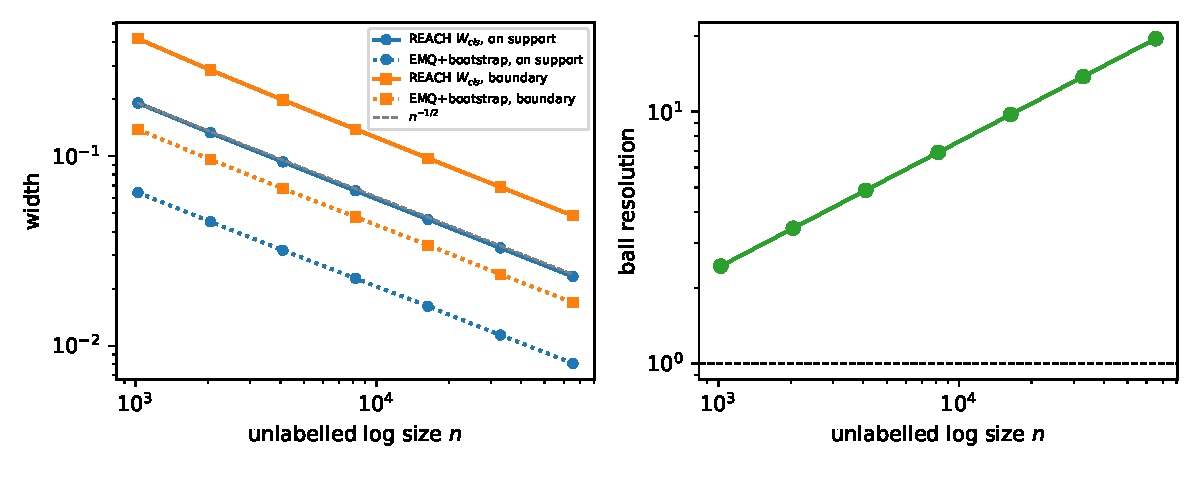
\includegraphics[width=.75\textwidth]{figures/fig2_wcls_vs_n.pdf}
\caption{Synthetic, world \emph{separated}. Left: $\Wcls$ (solid) and EMQ+bootstrap width (dotted)
against $n$; dashed slope $-1/2$. Right: ball resolution, which must exceed $1$ at the smallest $n$.}
\end{figure}

\paragraph{Second backbone.} With DINOv2 ViT-S/14 \citep{oquab2024dinov2} the head is $95.2\%$
accurate and the resolution gate reads $1.22$ (super4) and $1.75$ (ten sources). 13 of 13 registered
cells agree (12 of 13 with ten sources, the same saturated noise cell). The joint interval and the
constraint region cover in every seed in every label-shift and unseen-class arm; at $n=16{,}000$ their
widths are $0.69$ and $0.63$ (super4; $0.86$ and $0.72$ with ten sources), and the two-stage bootstrap
covers $0.74$ ($0.68$). Plug-in $\Wunk$ covers $0.89$ and $0.88$ when unseen classes are present; the
joint coverage interval covers in every seed. The corruption arm was not repeated for DINOv2.

\paragraph{Label noise (CLIP, super4).} Over $\eta\in\{0.025,\dots,0.3\}$ the joint interval and the
constraint region cover in every seed and both widen to $1.00$ (joint $0.92\to1.00$); the two-stage
bootstrap covers between $0.42$ and $0.73$.

\paragraph{Corruption--severity cells with joint coverage below $0.95$} (CLIP; coverage among answered
runs, and the rate at which the incompatibility test fires). \emph{four superclass sources}: elastic transform 5 (0.74, flag 0.35); frost 5 (0.90, flag 0.40); glass blur 1 (0.70, flag 0.90); glass blur 2 (0.70, flag 0.90); glass blur 3 (0.70, flag 0.85); jpeg compression 4 (0.95, flag 0.05); jpeg compression 5 (0.87, flag 0.35); motion blur 4 (0.94, flag 0.00); motion blur 5 (0.85, flag 0.45); pixelate 5 (0.80, flag 0.75).

\emph{ten class sources}: contrast 5 (0.80, flag 0.95); elastic transform 5 (0.92, flag 0.00); fog 5 (0.90, flag 0.00); frost 5 (0.94, flag 0.00); gaussian noise 2 (0.90, flag 0.00); gaussian noise 3 (0.81, flag 0.00); gaussian noise 4 (0.81, flag 0.00); gaussian noise 5 (0.80, flag 0.00); glass blur 1 (0.90, flag 0.00); glass blur 2 (0.90, flag 0.00); glass blur 3 (0.90, flag 0.00); glass blur 4 (0.86, flag 0.00); glass blur 5 (0.85, flag 0.00); impulse noise 4 (0.84, flag 0.00); impulse noise 5 (0.80, flag 0.00); jpeg compression 5 (0.94, flag 0.00); motion blur 5 (0.92, flag 0.00); pixelate 5 (0.93, flag 0.00); shot noise 3 (0.85, flag 0.00); shot noise 4 (0.83, flag 0.00); shot noise 5 (0.81, flag 0.00).

\paragraph{Where \cref{prop:c} stops: CIFAR-100.} Known sources are four trees (maple, oak, palm, pine)
and five vehicles, grouped into two sources; the novel source ($\delta=0.1$) is willow, a sibling of
the known trees, or whale. We registered that willow should show a smaller separation $s$, a flatter
$\Wunk$ slope and a wider final $\Wunk$ than whale. With 400 reference images per class the novel
row's radius alone is about $0.21$ and the resolution gate passes only for $n\ge8000$, so this arm is
descriptive. With CLIP all three predictions hold ($s=0.30$ vs $0.46$; slope $-0.02$, inside the
placebo band, vs $-0.09$; final width $0.57$ vs $0.51$). With DINOv2 only the slope prediction holds
($-0.03$ vs $-0.06$): in that encoder's cells willow is further from the known hull than whale
($s=0.35$ vs $0.32$). The joint novelty interval covers in all four runs. Whether a sibling class is
inside the support is a property of the representation, not of the label hierarchy.

\section{All pre-registered outcomes}
\label{app:outcomes}

\Cref{tab:outcomes-early,tab:outcomes-late} list every registered prediction with its outcome. Of the 24
directional claims registered for the attribution, Gaussian-feature and dose-response studies, 17 hold and
7 fail; the failures and their likely causes are plotted in \cref{fig:a1,fig:a2,fig:a3,fig:a4,fig:a5,fig:a6}.
Numbers are evaluation-seed means; brackets are 95\% bootstrap intervals.

\begin{table}[!htbp]
\centering\footnotesize
\caption{Registered outcomes of the tests in \cref{sec:exp-synthetic,sec:exp-real,sec:exp-blindspot,sec:exp-exchange}.}
\label{tab:outcomes-early}
\begin{tabular}{p{3.4cm}p{8.2cm}p{1.6cm}}
\toprule
test & outcome & verdict \\
\midrule
Synthetic response matrix & 23 of 25 cells agree; 12 baseline cells agree; of 7 non-trivial REACH cells 5 agree & 2 FAIL \\
\quad $\Wunk$, \emph{confounded} & registered ``no response''; slopes $-0.09$ (on support), $-0.04$ (boundary): attenuated, bounded below & FAIL \\
CIFAR-10 audit (CLIP, DINOv2) & 13/13 cells (super4); 12/13 (ten sources: saturated noise cell) & 1 FAIL each \\
CIFAR-100 limit arm & CLIP 3/3 predictions; DINOv2 1/3 (sibling class further from hull) & 2 FAIL \\
Acquisition under shift (v2) & REACH regret $0.084$ vs always-labels $0.010$ at 1:50 & FAIL \\
Exchange rate E1--E4 & all hold on synthetic and blind ResNet-50 & PASS \\
\bottomrule
\end{tabular}
\end{table}

\begin{table}[!htbp]
\centering\footnotesize
\caption{Registered outcomes of the attribution (v1, v2), Gaussian-feature (G) and dose-response (D)
studies. Pre-registrations: \texttt{real/bridge\_prereg.py}, \texttt{real/bridge2\_prereg.py} with
\texttt{real/bridge2\_amendment.py}, \texttt{real/gauss\_dose\_prereg.py}.}
\label{tab:outcomes-late}
\begin{tabular}{p{4.6cm}p{7.6cm}p{1.2cm}}
\toprule
claim & outcome & verdict \\
\midrule
v1 A1/A2: raw-width argmax beats budget-majority & regret $0.280$ vs $0.043$ (held-out), $0.356$ vs $0.015$ (label shift) & FAIL \\
v1 D1: $\Wcls$ falls with $\sigma(\hat A)$ & coefficient $+1.10$ $[1.02,1.23]$; confounded by $K$ (\cref{fig:a2}); B$'$ bound holds but never $<1$ & FAIL \\
v1 D2: $\Wunk$ falls with $s$ (40 candidates) & Spearman $-0.03$ $[-0.14,0.11]$; pooled across $K$ (\cref{fig:a3}) & FAIL \\
v1 D3: $\Wlab$ includes, tracks row error & inclusion $1.000$; positive in 21/24 & PASS \\
v1 D4: drift ratio $\rho$ vs inclusion, flag & Spearman $-0.72$, $+0.65$ (\cref{fig:a4}) & PASS \\
v2 P1: REACH-pin beats budget-majority (C10) & $-0.038$ $[-0.043,-0.033]$ & PASS \\
v2 P2/P3: same, classifier worlds; accuracy $\ge0.7$ & $-0.0075$ $[-0.010,-0.005]$; $0.91$ & PASS \\
v2 P4: same, $4\times$ acquisition & $-0.005$ $[-0.009,-0.002]$ & PASS \\
v2 P6: inclusion $\ge0.95$ & $1.000$ in every arm & PASS \\
G1: REACH-pin beats budget-majority & $-0.044$ $[-0.063,-0.026]$ & PASS \\
G2: inclusion & $1.000$ & PASS \\
G3: $\rho$ vs inclusion, flag & registered shifts too weak ($\rho\le0.35$), flag never fires (\cref{fig:a4}) & FAIL \\
G4a: $\Wcls$ falls with $\Delta$ & Spearman $-0.89$ $[-0.94,-0.77]$ & PASS \\
G4b: $\Wunk$ falls with $s$ & Spearman $+0.41$ $[0.28,0.57]$; $s\le0.2$ in every world (\cref{fig:a3}) & FAIL \\
Dcls-1: $n$-rate of $\Wcls$ in $[-0.75,-0.25]$ & $-0.40$ $[-0.41,-0.38]$ & PASS \\
Dcls-2: $\Wcls$ falls with $\sigma$, $K$ fixed & slope $-0.65$ $[-0.88,-0.52]$ (\cref{fig:a2}) & PASS \\
Dcls-3: lower probe mass, wider $\Wcls$ & 93\% of worlds & PASS \\
Dlab-1: $\Wlab$ monotone in $\eta$ (Spearman $=1$ in $\ge80\%$) & $67\%$; non-decreasing in 36/36, failures are ties at $\Wlab=1$ (\cref{fig:a5}) & FAIL \\
Dlab-2: label-interval inclusion & $1.000$ at every $\eta$ & PASS \\
Dlab-3: $\Wlab$ tracks realised error & Spearman $0.30$, positive in 36/36 & PASS \\
Dunk-1: $\Wunk$ falls with $s$, $K$ fixed & Spearman $-0.97$ $[-0.97,-0.94]$ (\cref{fig:a3}) & PASS \\
Dunk-2: no contraction at $s=0$; contraction for large $s$ & slopes $-0.095$ (bound $-0.1$, narrowly) and $-0.53$ & PASS \\
\bottomrule
\end{tabular}
\end{table}

\begin{figure}[!htbp]
\centering
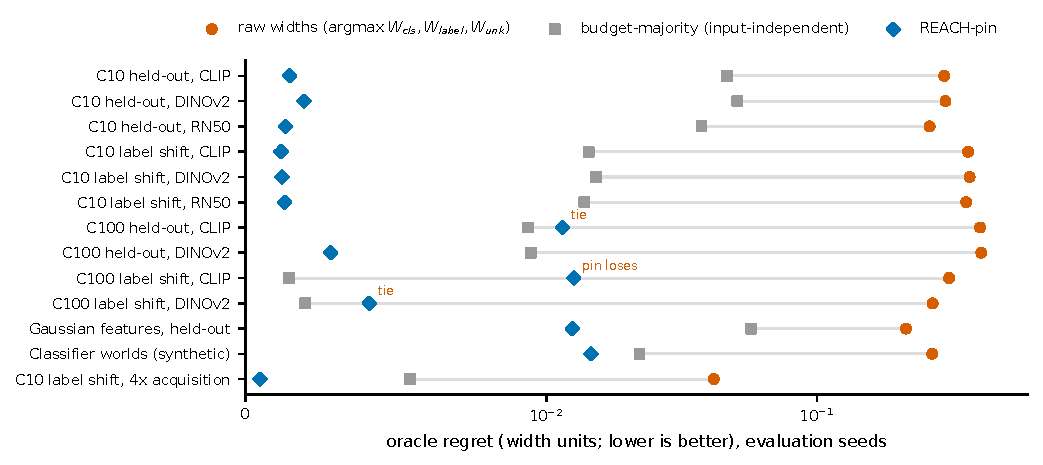
\includegraphics[width=.9\textwidth]{figures/figA1_attribution.pdf}
\caption{Oracle regret of naming the limiting source, per setting (log scale near $0$). REACH-pin beats
budget-majority on every CIFAR-10 setting, the Gaussian world, the classifier worlds and the $4\times$
acquisition outcome; on CIFAR-100, where the rows limit 90--99\% of inputs, it ties twice and loses once
(CI excluding $0$). The raw-width argmax is worst everywhere.}
\label{fig:a1}
\end{figure}

\begin{figure}[!htbp]
\centering
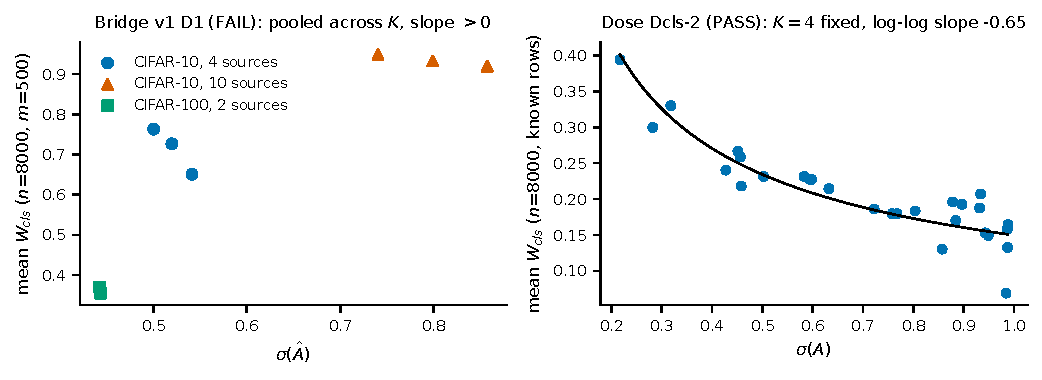
\includegraphics[width=.9\textwidth]{figures/figA2_sigma.pdf}
\caption{Prevalence width and distinguishability. Left (registered v1 D1, failed): pooling real settings
with different numbers of sources gives a positive slope, because ten-source settings have larger
$\sigma$ but smaller per-class mass. Right (Dcls-2, passed): with $K=4$ fixed, $\Wcls$ falls with $\sigma$.}
\label{fig:a2}
\end{figure}

\begin{figure}[!htbp]
\centering
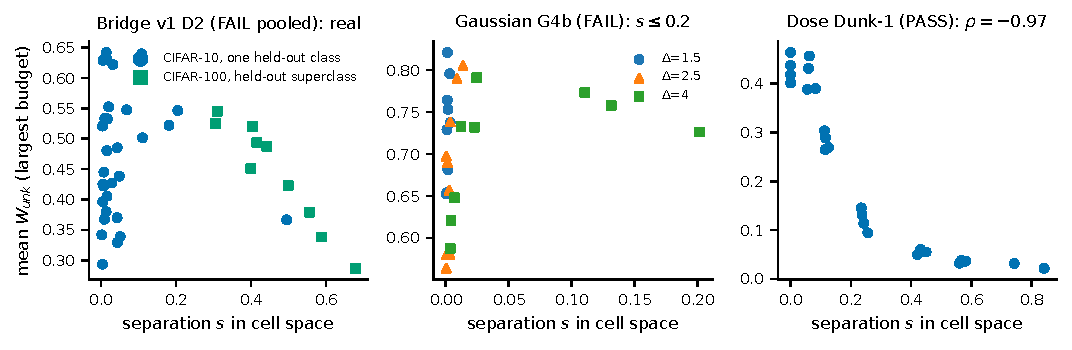
\includegraphics[width=\textwidth]{figures/figA3_separation.pdf}
\caption{Coverage width and separation in cell space. Left (v1 D2, failed pooled): real held-out classes;
within CIFAR-100 ($K=2$) the width falls with $s$. Centre (G4b, failed): Gaussian features; the head's PCA
projects the novel direction away, so $s\le0.2$ and the width follows how diffusely the novel class spreads.
Right (Dunk-1, passed): categorical worlds with $K=4$ fixed.}
\label{fig:a3}
\end{figure}

\begin{figure}[!htbp]
\centering
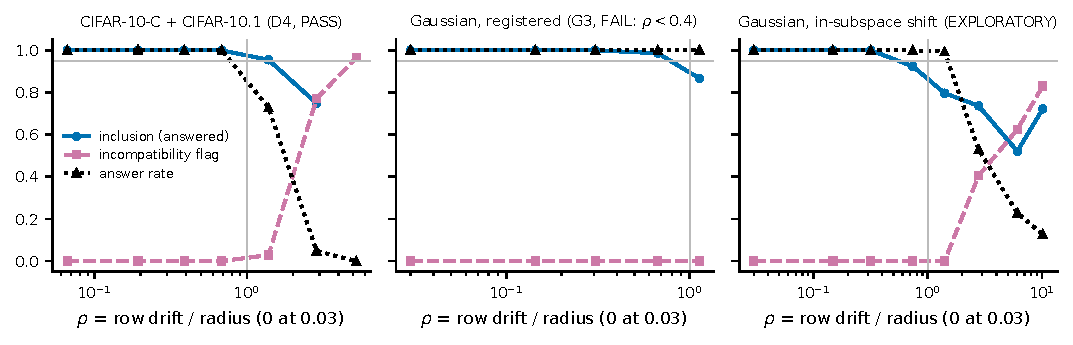
\includegraphics[width=\textwidth]{figures/figA4_shift.pdf}
\caption{Inclusion among answered runs, incompatibility-flag rate and answer rate against $\rho$, the row
drift in units of the ball radius (binned). Left: CIFAR-10-C and CIFAR-10.1 (registered, passed). Centre:
registered Gaussian shifts, too weak to reach $\rho=1$ (failed). Right (exploratory, not registered):
shift inside the head's subspace; inclusion falls to $0.92$ at $\rho\in(0.5,1]$ and $0.80$ at $\rho\in(1,2]$
before the flag fires.}
\label{fig:a4}
\end{figure}

\begin{figure}[!htbp]
\centering
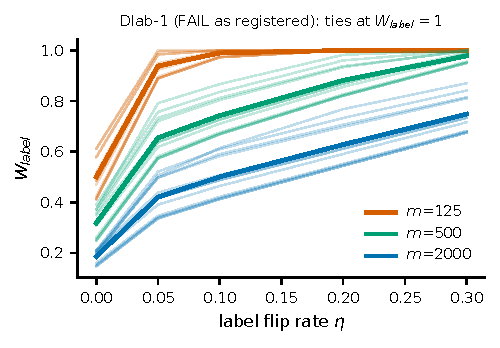
\includegraphics[width=.5\textwidth]{figures/figA5_label_noise.pdf}
\caption{Label width against label noise (Dlab-1, failed as operationalised). Thin lines: worlds; thick:
means. The width never decreases in $\eta$; at $m=125$ it saturates at $1$, and the resulting ties fail the
registered ``Spearman $=1$'' criterion.}
\label{fig:a5}
\end{figure}

\begin{figure}[!htbp]
\centering
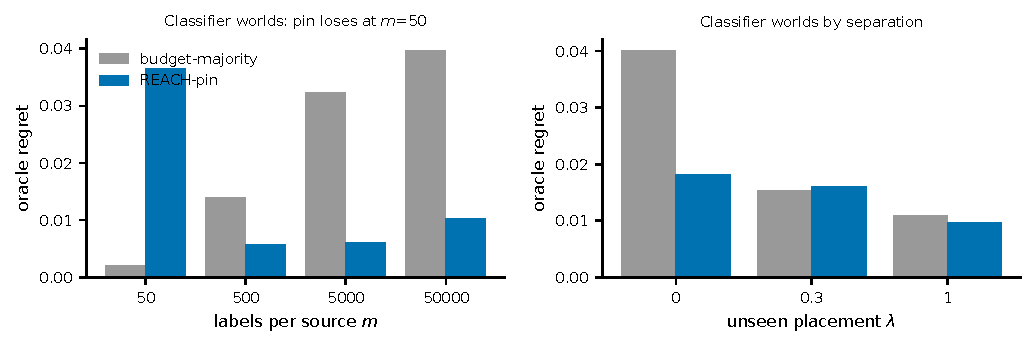
\includegraphics[width=.9\textwidth]{figures/figA6_pin_limits.pdf}
\caption{Where REACH-pin does not help (classifier worlds). Left: with $m=50$ labels per source the rows
limit almost every input and the pinned rows are poor, so pinning loses to budget-majority. Right: by
placement of the unseen source.}
\label{fig:a6}
\end{figure}

\clearpage
\section{Pre-registration and deviations}
\label{app:deviations}

Expected outcomes were committed in code before each test ran, and run manifests record each file's
SHA-256. These are self-registrations in a local repository without third-party timestamps, so a
reader can check consistency between files, hashes and results but not the order of events; we state
the order below.
\begin{itemize}
\item Synthetic study: \texttt{train/expectations.py} (7a97650e\ldots), before the first run.
\item Real audit: \texttt{real/expectations.py}, in four states: 068095ec\ldots{} (before the
Dirichlet, label-noise and $\delta=0$ runs, written after earlier fixed-skew runs had been inspected);
9a09b019\ldots{} (adds DINOv2 and CIFAR-100, before those features existed); 761495e4\ldots{} (adds the
CIFAR-100 grouping change and the joint coverage interval, after the first CIFAR-100 and DINOv2 runs);
add1ccd3\ldots{} (adds the two baselines of \cref{sec:exp-real}, after a one-seed smoke test, before
the reported reruns).
\item Acquisition test, version 1: \texttt{real/blindspot\_prereg.py} (e699e72d\ldots). Its header
says 2026-10-03; it was written on 2026-10-02 at 19:32, one minute before the test code and after the
corruption audit had shown the incompatibility flag rising with severity, so the off-frame rule was
not blind to that link.
\item Acquisition test, version 2: \texttt{real/blindspot\_prereg\_v2.py} (2fdecf48\ldots), written
2026-10-02 23:09 after version 1's results and its review, before any version-2 code.
\item Exchange-rate test: \texttt{real/exchange\_prereg.py} (a70683e3\ldots), 2026-10-03 06:52.
\item Attribution v1: \texttt{real/bridge\_prereg.py} (cd88f846\ldots), 2026-10-03 19:37, before its code.
\item Attribution v2: \texttt{real/bridge2\_prereg.py} (d8e97dab\ldots), 2026-10-04 14:58, after the v1
results and before any v2 code; amendment \texttt{real/bridge2\_amendment.py} (9f4a189d\ldots), 15:01.
\item Gaussian world and dose-responses: \texttt{real/gauss\_dose\_prereg.py} (fbbfe136\ldots), 2026-10-04
15:18, after the v2 results and before any code for these tests.
\end{itemize}
Deviations, all disclosed:
\begin{enumerate}
\item The coordinate-box ball was replaced by the exact ball after exploratory real runs were close to
vacuous with it.
\item The joint interval was introduced after exploratory real runs showed plug-in $\Wcls$
under-covering, and the joint coverage interval after DINOv2 runs showed the same for plug-in $\Wunk$.
Both were then evaluated on the same seeds and the same test pool used in their design; their real-data
coverage is therefore not a held-out confirmation.
\item A region-labelling error under grouped sources mislabelled the outlier cell; all grouped runs
were repeated.
\item Coverage is judged at tolerance $10^{-6}$, the solver's accuracy, after $10^{-9}$-level solver
output was seen to fail a $10^{-9}$ test where the exact extremum is $0$. The synthetic study keeps the
original $10^{-9}$ tolerance with the coordinate-box solver.
\item The first label-noise radius had an avoidable $\sqrt K$ factor and was replaced before the reported
runs.
\item The CIFAR-100 grouping was changed after singleton sources failed the resolution gate at every
$n$; the CIFAR-100 slopes are fitted over grid points where the gate still fails ($n\le4000$).
\item Acquisition test version 1 had two rule defects (a non-finite predicted log gain, when the
hypothetical ball at the same histogram and smaller radius was empty, defaulted to labels; the label
gain priced 25 clean labels per source while the action bought 100 shifted ones), tuned the baseline
for matching accuracy rather than regret, and resampled (split, seed) episodes where its registration
named seeds. Version 2 fixes all four; version 1 is superseded and its results are not used.
\item Corruption runs use 20 seeds per corruption and severity, not 50. Runs whose ball is empty
abstain; coverage is reported among answered runs and unconditionally.
\item The version-2 acquisition rule, as registered, cannot recommend labels in a compatible frame
(\cref{sec:exp-blindspot}); we noticed this only after its run. We report the registered rule unchanged.
\item The third state of \texttt{real/expectations.py} carries a hand-written time (``$\sim$23:25'') that
disagrees with its file time (23:12); the order relative to the runs is unaffected.
\item Exchange-rate test: \texttt{real/exchange\_prereg.py} (a70683e3\ldots) was written 2026-10-03 06:52,
before its code and before any ResNet-50 feature existed. The first ResNet-50 run crashed in the ensemble
baseline (every member's resampled log was incompatible with the estimated rows); the fix, which marks
such episodes' MI as undefined and places them in the top tercile, was made before any ResNet-50 result
existed. The synthetic and CLIP runs did not reach that case, and rerunning both with the final code
reproduces their results (synthetic bit-exactly, CLIP to $10^{-15}$). The crashed run's log is not
released.
\item Attribution v1: the CIFAR-100 class ids were not sorted, which crashed the head fit; the
domain-shift arm crashed on an unguarded solver failure. Both were fixed and rerun before any result of
those arms existed. Units whose every probe abstains have no inclusion rate and are excluded from the D4
correlation (46 of 304). A comparison of a logistic map of the widths with budget-majority was added after
the CIFAR-10 results were seen and is exploratory.
\item REACH-pin replaces the raw-width argmax as the attribution rule after the v1 failure. It was
registered before any v2 code and evaluated on fresh real seeds; v1 is reported unchanged.
\item Attribution v2 amendment: the registered dense synthetic worlds (rows drawn from Dirichlet
distributions over 10 or 50 cells) gave total widths of about $1$ at every budget, so they were replaced by
classifier-like worlds and larger label budgets before any claim was scored. The only data seen were
smoke runs and a width probe on single worlds that used seed 5, an evaluation seed. The amendment's
docstring states ``$\sim$15:40''; the file was written at 15:01, before the run launched.
\item The in-subspace Gaussian shift (\cref{fig:a4}, right) was run after the registered shift design
failed and is exploratory.
\end{enumerate}
